%% NeuralSS manuscript for the Journal of Real-Time Image Processing (Springer).
%% Template: Springer Nature LaTeX template v3.1 (December 2024), two-column option [iicol] as the journal recommends.
%% Variants: main-anonymised.tex (\Anonymised), main-title-page.tex (\TitlePage), main-no-references.tex (\NoReferences).
%% Supplementary material (Online Resource 1): supplementary.tex, labels referenced with the S- prefix.
%% Build: python tools/build_paper.py from the repository root (see paper/README.md).
\RequirePackage{xr-hyper}
\documentclass[pdflatex,sn-mathphys-num,iicol]{sn-jnl}

%% Shared preamble of the manuscript (main.tex) and the supplementary material (supplementary.tex).
%% Loaded after \documentclass. Both files load xr-hyper with \RequirePackage before \documentclass,
%% because sn-jnl.cls loads hyperref itself.

\usepackage{graphicx}%
\usepackage{multirow}%
\usepackage{amsmath,amssymb,amsfonts}%
\usepackage{xcolor}%
\usepackage{textcomp}%
\usepackage{booktabs}%
\usepackage{tikz}%
\usetikzlibrary{positioning,arrows.meta,fit}%
\usepackage[capitalise,nameinlink]{cleveref}%
\hypersetup{bookmarksnumbered=true}
\usepackage{xurl}% break long URLs in the reference list
\newcommand{\burl}[1]{\url{#1}}% sn-mathphys-num prints URL fields in sans serif without a link

%% Variant suffix used to pair each document with its counterpart (main / supplementary)
\ifdefined\Anonymised \def\Variant{-anonymised}\else \def\Variant{}\fi

\newcommand{\Sys}{NeuralSS}
\newcommand{\tier}[1]{\texttt{#1}}
\newcommand{\RepoURL}{\url{https://github.com/parthmital/High-Throughput-Neural-Super-Sampling}}

%% Results. Every number taken from a run is a key in results-values.tex, which
%% tools/build_paper_results.py generates from the notebooks' metric files. Never type such a number.
%%   \Res{key}          the value of key
%%   \ResDiff{a}{b}     signed difference a - b (computed by the generator, which scans the .tex files)
%%   \ResAbsDiff{a}{b}  unsigned difference |a - b|
%%   \ResRatio{a}{b}    ratio a / b
%% A missing key prints a red ??key in the PDF (check_paper.py fails on ??) and a LaTeX warning.
\makeatletter
\newcommand{\SetResult}[2]{\expandafter\def\csname nss@res@#1\endcsname{#2}}
\newcommand{\Res}[1]{%
  \ifcsname nss@res@#1\endcsname\csname nss@res@#1\endcsname
  \else\textbf{\textcolor{red}{??\detokenize{#1}}}\PackageWarning{neuralss}{Missing result key #1}\fi}
\newcommand{\ResDiff}[2]{\Res{diff:#1:#2}}
\newcommand{\ResAbsDiff}[2]{\Res{absdiff:#1:#2}}
\newcommand{\ResRatio}[2]{\Res{ratio:#1:#2}}
\makeatother
\InputIfFileExists{results-values}{}{\PackageWarning{neuralss}{results-values.tex missing, run tools/build_paper_results.py}}

%% Status of a finding (used in the supplementary material, defined in its Section S1):
%%   \Confirmed     holds in every available run and is not sensitive to the details expected to change
%%   \Preliminary   measured in one run (one seed, one budget), may change with further runs
%%   \Observation   qualitative or from few samples, from inspection of outputs rather than a test statistic
%%   \UnderRevision describes a component or protocol that the next pipeline version is expected to change
\definecolor{nssConfirmed}{RGB}{0,110,60}
\definecolor{nssPreliminary}{RGB}{170,100,0}
\definecolor{nssObservation}{RGB}{40,80,170}
\definecolor{nssRevision}{RGB}{170,30,30}
\newcommand{\nssTag}[2]{\textsf{\footnotesize\textbf{\textcolor{#1}{[#2]}}}}
\newcommand{\Confirmed}{\nssTag{nssConfirmed}{Confirmed}}
\newcommand{\Preliminary}{\nssTag{nssPreliminary}{Preliminary}}
\newcommand{\Observation}{\nssTag{nssObservation}{Observation}}
\newcommand{\UnderRevision}{\nssTag{nssRevision}{Under revision}}
%% A place that still needs a verified citation. Prints a red marker, so it cannot survive a final build.
\newcommand{\NeedsCite}[1]{\textbf{\textcolor{red}{[??citation: #1]}}\PackageWarning{neuralss}{Citation needed: #1}}

\externaldocument[S-]{supplementary\Variant}

\ifdefined\NoReferences
\makeatletter
\renewenvironment{thebibliography}[1]{\setbox0=\vbox\bgroup\list{}{\usecounter{enumiv}}}{\endlist\egroup}
\makeatother
\fi

\raggedbottom

\begin{document}

\title[Vendor-neutral neural super-resolution and frame generation]{One network for renders and video: vendor-neutral neural temporal super-resolution and low-latency frame generation trained on commodity cloud GPUs}

\ifdefined\Anonymised
\author*{\fnm{Anonymous} \sur{Author}}\email{anonymous@example.org}
\affil*{\orgname{Anonymous institution}}
\else
\author*{\fnm{Parth} \sur{Mital}}\email{parth.mital2023@vitstudent.ac.in}
\affil*{\orgdiv{School of Computer Science and Engineering}, \orgname{Vellore Institute of Technology}, \orgaddress{\city{Vellore}, \postcode{632014}, \state{Tamil Nadu}, \country{India}}}
\fi

\abstract{Neural upscaling and frame generation now set image quality in many games, but the strongest commercial systems need one vendor's recent GPUs, and research systems need engine data that ordinary video lacks. We present \Sys{}, an open system that serves both cases with one model per task. Its temporal super-resolution network is a recurrent, re-parameterisable convolutional network with a built-in motion estimator that runs only when the engine supplies no motion vectors. Its frame-generation network fine-tunes the open RIFE 4.26 interpolation network, adds engine hints through zero-initialised channels, extrapolates with a late-latched camera prior and blends user-interface pixels towards the newest real frame. Both are trained in \Res{tsr.summary.run_hours} and \Res{fg.summary.run_hours} hours on two NVIDIA T4 GPUs from public datasets, after copy detection that left no duplicate across splits, and both export to ONNX. On five test suites the 3x super-resolution student (\Res{tsr.model_tiers.low.3.gmac_per_frame_1080p} GMAC per 1080p frame) beats bicubic upscaling on ordinary video by \ResAbsDiff{tsr.test_results.vimeo1080p.plain.3.student_s3.psnr_y}{tsr.test_results.vimeo1080p.plain.3.bicubic.psnr_y} to \ResAbsDiff{tsr.test_results.synthetic-game.plain.3.student_s3.psnr_y}{tsr.test_results.synthetic-game.plain.3.bicubic.psnr_y} dB PSNR-Y and an analytic temporal anti-aliasing upscaler by \ResAbsDiff{tsr.test_results.tartanair.engine.3.student_s3.psnr_y}{tsr.test_results.tartanair.engine.3.analytic_taau.psnr_y} to \ResAbsDiff{tsr.test_results.synthetic-game.engine.3.student_s3.psnr_y}{tsr.test_results.synthetic-game.engine.3.analytic_taau.psnr_y} dB with engine data, with lower temporal-change error. The largest frame-generation tier beats unchanged RIFE 4.26 on the Middlebury interpolation set (\Res{mb.middlebury_psnr.mean.high.psnr} against \Res{mb.middlebury_psnr.mean.rife_4_26.psnr} dB) and frame repetition in extrapolation by \ResAbsDiff{fg.test_per_sample.vimeo1080p_native.extrap.plain.high.psnr}{fg.test_per_sample.vimeo1080p_native.extrap.plain.repeat.psnr} to \ResAbsDiff{fg.test_per_sample.tartanair.extrap.plain.high.psnr}{fg.test_per_sample.tartanair.extrap.plain.repeat.psnr} dB, but the \Res{fg.model_tiers.low.gmac_per_1080p_frame}-GMAC tier is still \ResAbsDiff{mb.middlebury_psnr.mean.low.psnr}{mb.middlebury_psnr.mean.rife_4_26.psnr} dB below RIFE on Middlebury, the cut detector false-alarms on multi-frame gaps, and eager PyTorch on a T4 needs \Res{tsr.latency.student_s3.3.1920x1080.t4_mean_ms} and \Res{fg.latency.student.1920x1080.t4_mean_ms} ms per 1080p frame, above real-time budgets. We report these limits with the gains.}

\keywords{Temporal super-resolution, Frame generation, Video frame interpolation, Real-time rendering, Latency, Efficient neural networks}

\pdfbookmark[1]{Title}{title}
\maketitle

\ifdefined\TitlePage
\section*{Corresponding author}
\pdfbookmark[1]{Corresponding author}{corresponding}
\noindent Parth Mital\\
School of Computer Science and Engineering, Vellore Institute of Technology\\
Vellore 632014, Tamil Nadu, India\\
E-mail: \href{mailto:parth.mital2023@vitstudent.ac.in}{\nolinkurl{parth.mital2023@vitstudent.ac.in}}
\expandafter\endinput\fi

\section{Introduction}\label{sec:intro}

Games increasingly render fewer pixels than they display. A temporal upscaler reconstructs each output frame from a jittered low-resolution render and the history of earlier frames, and a frame generator inserts synthetic frames between rendered ones. Neural versions of both now ship in vendor SDKs, but the strongest paths need recent hardware of one vendor: DLSS 4 multi-frame generation relies on RTX 50 Series GPUs\footnote{\url{https://research.nvidia.com/labs/adlr/DLSS4}, accessed 8 November 2026.}, and AMD's machine-learning upscaling and frame generation require RDNA 4 GPUs, with analytical fallbacks on older ones\footnote{\url{https://gpuopen.com/learn/amd-fsr-redstone-developers-neural-rendering/}, accessed 8 November 2026.}. Intel's XeSS super-resolution runs on any GPU with Shader Model 6.4\footnote{\url{https://github.com/intel/xess}, accessed 8 November 2026.}. Research systems are open but assume a full set of engine buffers \cite{xiao2020nsrr,zhong2023fusesr,guo2021extranet}, so they cannot serve captured or streamed video, where only colour exists. Video frame interpolation networks such as RIFE \cite{huang2022rife} work from colour alone but ignore the motion vectors, depth and user-interface (UI) layers that an engine can provide, and they do not extrapolate.

This paper asks whether one compact model per task can serve engine renders with motion vectors and plain video without them, at a cost that fits integrated and entry-level GPUs, when trained with free cloud compute and public data only. Each network has tiers sized in multiply-accumulates (MAC) per 1080p output frame. Frame generation is designed around input latency rather than frame rate, so it supports extrapolation, which holds no rendered frame back. Both networks reduce to convolutions, pixel shuffles and bilinear warps that export to ONNX.

The contributions are:
\begin{enumerate}
\item A recurrent temporal super-resolution (TSR) network with a built-in motion estimator, trained on mixed render-like and plain-video degradations so that one model serves both, with tiers from \Res{tsr.model_tiers.igpu.3.gmac_per_frame_1080p} to \Res{tsr.model_tiers.teacher.3.gmac_per_frame_1080p} GMAC per 1080p frame at 3x (\cref{sec:tsr}).
\item A frame-generation (FG) network that fine-tunes RIFE 4.26 and adds engine hints through zero-initialised channels. The fresh IFNet blend reproduces RIFE 4.26, but the fresh head mixes the newest real frame in at UI weight $\sigma(-4)\approx0.018$. The network adds a learned UI weight, a late-latched camera prior for extrapolation and a scene-cut gate (\cref{sec:fg}).
\item A leakage-audited data pipeline over \Res{data.split_report.items} public items and an evaluation protocol that tests every suite in an engine mode and a plain-video mode, with temporal, UI, cut and latency measures (\cref{sec:data,sec:setup}).
\item Measurements on two Kaggle T4 GPUs that include the failures: the small FG tiers stay below RIFE, the plain-video cut gate false-alarms, and eager latency exceeds the tier budgets (\cref{sec:results,sec:discussion}).
\end{enumerate}
\Cref{fig:overview} summarises both networks.

\begin{figure*}[!t]
\centering
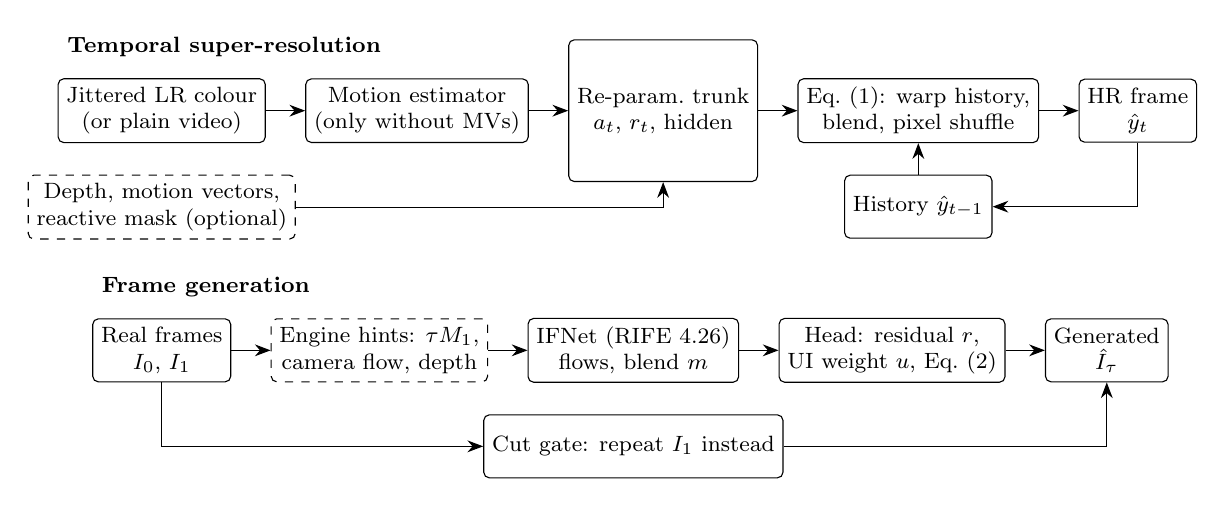
\begin{tikzpicture}[font=\footnotesize, node distance=4mm and 5mm,
  box/.style={draw, rounded corners=2pt, align=center, minimum height=8mm, inner sep=3pt},
  opt/.style={box, dashed},
  arr/.style={-{Stealth[length=2mm]}}]
\node[box] (lr) {Jittered LR colour\\(or plain video)};
\node[opt, below=of lr] (eng) {Depth, motion vectors,\\reactive mask (optional)};
\node[box, right=of lr] (est) {Motion estimator\\(only without MVs)};
\node[box, right=of est, minimum height=18mm] (trunk) {Re-param.\ trunk\\$a_t$, $r_t$, hidden};
\node[box, right=of trunk] (acc) {Eq.~(1): warp history,\\blend, pixel shuffle};
\node[box, right=of acc] (hr) {HR frame\\$\hat{y}_t$};
\node[box, below=of acc] (hist) {History $\hat{y}_{t-1}$};
\draw[arr] (lr) -- (est); \draw[arr] (est) -- (trunk); \draw[arr] (eng.east) -| (trunk.south);
\draw[arr] (trunk) -- (acc); \draw[arr] (acc) -- (hr); \draw[arr] (hist) -- (acc);
\draw[arr] (hr.south) |- (hist.east);
\node[box, below=10mm of eng] (pair) {Real frames\\$I_0$, $I_1$};
\node[opt, right=of pair] (hint) {Engine hints: $\tau M_1$,\\camera flow, depth};
\node[box, right=of hint] (ifn) {IFNet (RIFE 4.26)\\flows, blend $m$};
\node[box, right=of ifn] (head) {Head: residual $r$,\\UI weight $u$, Eq.~(2)};
\node[box, right=of head] (out) {Generated\\$\hat{I}_\tau$};
\node[box, below=of ifn] (cut) {Cut gate: repeat $I_1$ instead};
\draw[arr] (pair) -- (hint); \draw[arr] (hint) -- (ifn); \draw[arr] (ifn) -- (head); \draw[arr] (head) -- (out);
\draw[arr] (pair.south) |- (cut.west); \draw[arr] (cut.east) -| (out.south);
\node[anchor=west, font=\footnotesize\bfseries] at ([yshift=4mm]lr.north west) {Temporal super-resolution};
\node[anchor=west, font=\footnotesize\bfseries] at ([yshift=4mm]pair.north west) {Frame generation};
\end{tikzpicture}
\caption{Overview of the two networks. Dashed boxes are engine inputs that are used when present and dropped at random in training. Both networks reduce to convolutions, pixel shuffles and bilinear warps for ONNX export}\label{fig:overview}
\end{figure*}

\section{Related work}\label{sec:related}

\emph{Temporal anti-aliasing and upscaling.} Temporal anti-aliasing reprojects an accumulated history with motion vectors and rectifies it against the current frame's neighbourhood to suppress ghosting, and temporal upsampling extends the same idea to lower render resolutions \cite{yang2020taasurvey}.
\emph{Neural supersampling for rendering.} NSRR reconstructs high-resolution frames from the colour, depth and dense motion vectors of the current and previous frames \cite{xiao2020nsrr}. Later work combines denoising and supersampling in a temporally stable network \cite{thomas2022denoise}, reduces cost on a new gaming dataset \cite{mercier2023qrisp}, fuses high-resolution G-buffers with low-resolution colour \cite{zhong2023fusesr}, demodulates lighting from materials \cite{li2024demodulation} and decouples G-buffer guidance \cite{zheng2025rdg}. All assume engine buffers at inference. Our TSR network uses them when present and estimates motion itself when they are absent.

\emph{Frame generation for rendering.} Interpolation for rendered content can use auxiliary buffers \cite{briedis2021rendered}, but it holds a rendered frame back. Extrapolation avoids that latency: ExtraNet uses G-buffers of the new frame and in-paints disocclusions \cite{guo2021extranet}, ExtraSS joins extrapolation with supersampling \cite{wu2023extrass}, space-time supersampling treats both in one network \cite{he2024stss}, GFFE removes the need for the new frame's G-buffers \cite{wu2024gffe}, and Mob-FGSR targets mobile GPUs \cite{yang2024mobfgsr}.

\emph{Video frame interpolation.} RIFE estimates intermediate flows coarse to fine with an IFNet at an arbitrary time step and runs in real time \cite{huang2022rife}. IFRNet \cite{kong2022ifrnet}, FILM \cite{reda2022film} and EMA-VFI \cite{zhang2023emavfi} trade more computation for accuracy or large motion. Logos, UI and subtitles break interpolation, and a discontinuity map with figure-text mixing copies such regions from the previous frame instead of interpolating them \cite{lee2023discontinuity}. We build on RIFE 4.26 because its weights are open and it is cheap enough to tier.

\emph{Efficient networks and temporal metrics.} Structural re-parameterisation trains multi-branch blocks and deploys one $3\times3$ convolution \cite{ding2021repvgg,zhang2021ecbsr}, and sub-pixel convolution upsamples cheaply \cite{shi2016espcn}. Recurrent video super-resolution propagates features across frames \cite{chan2022basicvsrpp}. TecoGAN defines the tOF and tLP temporal metrics we report \cite{chu2020tecogan}.

\section{Data and leakage control}\label{sec:data}

Training and test data come only from public sources: DIV2K \cite{agustsson2017div2k} and other high-resolution stills, 1080p game frames, REDS \cite{nah2019reds}, Vimeo-90K septuplets and triplets \cite{xue2019vimeo}, MPI Sintel with exact flow and occlusion \cite{butler2012sintel}, TartanAir with exact flow and depth from Unreal Engine environments \cite{wang2020tartanair}, CARLA \cite{dosovitskiy2017carla} renders from GameIR with native 720p and 1440p frames \cite{zhou2024gameir}, the Vid4 sequences (calendar, city, foliage and walk) evaluated by Liu and Sun \cite{liu2014vid4}, and 1080p Vimeo videos. Low-resolution inputs are generated from high-resolution frames, so every sample has ground truth. Online Resource 1 (\cref{S-sec:data-sources}) lists every source and licence.

Copy detection runs in two stages, because global similarity alone cannot tell the same picture from a similar one. Candidates are the \Res{data.config.cfg.dedup.k} nearest neighbours of each keyframe by self-supervised DINOv2-small embeddings outside its leakage group plus perceptual-hash pairs, and a candidate becomes a duplicate edge when SIFT matches \cite{lowe2004sift} with the ratio test and one RANSAC affine fit \cite{fischler1981ransac} cover at least \Res{data.dedup_calibration.verify.t_cells} cells of an $8\times8$ grid, or when its embedding or hash similarity passes a stricter threshold. Thresholds are calibrated on \Res{data.config.cfg.calibration_pairs} synthetic copies against \Res{data.calibration_scores.0.random.n} random and \Res{data.calibration_scores.0.hard.n} hard negatives (recall \Res{data.dedup_calibration.rule.recall} at precision \Res{data.dedup_calibration.rule.precision}). Leakage groups (a video, a Sintel scene family, a TartanAir environment, a CARLA town) are the unit of the split, and any training item linked to a test item by a duplicate edge is dropped. An audit then compares every validation keyframe with its \Res{data.config.cfg.dedup.audit_k} nearest training keyframes, and every test keyframe with its nearest training and validation keyframes, by cosine similarity and by pHash.

On \Res{data.split_report.items} items the split is \Res{data.split_report.split_counts.train} training, \Res{data.split_report.split_counts.val} validation and \Res{data.split_report.split_counts.test} test items, with \Res{data.split_report.split_counts.drop} dropped and \Res{data.split_report.split_counts.filtered} filtered for quality. The audit took \Res{data.split_report.audit_rounds} rounds: the first found duplicates that the search had missed, and the last found none (Online Resource 1, \cref{S-sec:data-copy,S-sec:data-audit}).

A GPU renderer adds synthetic game-like sequences with exact ground truth. A background and a foreground layer with procedural alpha (blobs, wires one or two texels wide, fences) move on their own affine paths at four speed classes (static, slow, medium, fast) with optional reversal. Particles write no motion vectors and set a reactive mask, as in real engines. Low-resolution frames take one jittered sample per pixel at Halton (2, 3) offsets without mip filtering, so thin geometry aliases, and targets use four samples per pixel. For FG the renderer adds HUD tiles, subtitle changes, menus and scene cuts (\cref{S-sec:data-synth}).

\section{Temporal super-resolution}\label{sec:tsr}

\emph{Inputs.} At render resolution $h\times w$ the network receives the jittered colour, depth and normals derived from it, motion vectors to the previous frame, a depth-based disocclusion cue, the reactive mask, exposure and jitter offsets, flags for depth availability and motion quality (1 for exact vectors, 0.5 for RAFT, 0.25 for the built-in estimator, 0 for none), an input-kind flag (render or video), the previous output warped by the motion vectors and folded to render resolution by space-to-depth, and a warped recurrent hidden state.

\emph{Motion without engine data.} Every tier contains a three-level IFNet motion estimator \cite{huang2022rife} that computes motion vectors from the previous and current colour frames whenever a sample has none. Its output enters the trunk with motion quality 0.25. It is supervised by exact or RAFT (small model) \cite{teed2020raft} motion, and during the first quarter of training samples without motion vectors warp the history with the label motion at a falling probability (teacher forcing), so that the trunk does not learn to distrust history while the estimator is poor. With engine motion vectors the estimator is skipped.

\emph{Trunk and output.} The trunk is a chain of re-parameterisable blocks (a $3\times3$, a $1\times1$, an identity and fixed Sobel and Laplacian filters with learned projections) folded into one $3\times3$ kernel \cite{zhang2021ecbsr}, with an optional half-resolution U-Net level. In each block the $1\times1$ and edge-projection branches start with zero weights (their biases keep the default initialisation), which kept activations bounded in FP16. The network predicts a per-pixel history weight $a_t$ and a residual $r_t$ at render resolution, unfolds them by pixel shuffle \cite{shi2016espcn}, and forms
\begin{equation}
\hat{y}_t = a_t \odot \mathcal{W}(\hat{y}_{t-1}, \mathbf{m}_t) + (1-a_t) \odot \mathcal{U}(x_t) + r_t ,\label{eq:tsr}
\end{equation}
where $\mathcal{W}$ warps by the upsampled motion $\mathbf{m}_t$ and $\mathcal{U}$ is a jitter-aware bilinear upsampling of the colour $x_t$. A refinement at output resolution follows in all tiers but the smallest, whose last layer starts at zero. \Cref{eq:tsr} is a learned form of temporal accumulation with rectification: $a_t$ should approach 0 at disocclusions and particles and 1 on static content. After a reset $a_t=0$.

\emph{Training.} A share \Res{tsr.config.cfg.p_real} of each batch is real video and the rest is synthetic. A share \Res{tsr.config.cfg.p_video_synth} of synthetic and \Res{tsr.config.cfg.p_video_real} of real samples become plain video: anti-aliased bicubic, bilinear or area downscaling, blur, noise and 8-bit quantisation, without jitter, depth or reactive mask. Of these, a share \Res{tsr.config.cfg.p_video_mv} keep block-averaged motion vectors of quality at most 0.5, and the others have none, so the estimator runs. Every sample loses its motion vectors with probability \Res{tsr.config.cfg.p_drop_mv} and its depth with probability \Res{tsr.config.cfg.p_drop_depth}. Six-frame unrolls on $192\times192$ output patches are the default, and every \Res{tsr.config.cfg.long_every}-th step is a \Res{tsr.config.cfg.long_t}-frame synthetic unroll at $96\times96$ so that static scenes keep converging. The per-frame loss is a Charbonnier penalty plus \Res{tsr.config.cfg.w_grad} times a gradient loss, \Res{tsr.config.cfg.w_fft} times an L1 loss on Fourier magnitudes, \Res{tsr.config.cfg.w_lpips} times LPIPS \cite{zhang2018lpips} on the last frame, and \Res{tsr.config.cfg.w_temporal} times a temporal-change loss over pixels visible in both frames, plus \Res{tsr.config.cfg.w_flow} times the motion loss. Training uses AdamW \cite{loshchilov2019adamw}, FP16 autocast with loss scaling \cite{micikevicius2018mixed}, a cosine schedule over a wall-clock budget, and an exponential moving average of the weights. Distillation from the teacher gave no measurable gain in earlier runs and is off (weight \Res{tsr.config.cfg.w_distill}). Online Resource 1 (\cref{S-sec:tsrm}) gives every input, equation and hyperparameter.

\Cref{tab:tiers} lists the tiers. The teacher is the same architecture at 64 channels and serves as the quality ceiling.

\begin{table}[!t]
\caption{Network tiers: fused parameters, multiply-accumulates per 1080p output frame (GMAC, warps excluded) and measured T4 latency (fused FP16, eager PyTorch, cuDNN autotuning). TSR figures are for 3x and include the motion estimator, which runs only without engine motion vectors (latency with engine vectors in brackets).}\label{tab:tiers}
\begin{tabular*}{\columnwidth}{@{\extracolsep\fill}llrrr}
\toprule
Task & Tier & Params & GMAC & T4 ms \\
\midrule
TSR & \tier{igpu} & \Res{tsr.model_tiers.igpu.3.fused_params} & \Res{tsr.model_tiers.igpu.3.gmac_per_frame_1080p} & \Res{tsr.latency.igpu_s3.3.1920x1080.t4_mean_ms} (\Res{tsr.latency.igpu_s3.3.1920x1080.t4_mean_ms_engine_mv}) \\
 & \tier{low} & \Res{tsr.model_tiers.low.3.fused_params} & \Res{tsr.model_tiers.low.3.gmac_per_frame_1080p} & \Res{tsr.latency.student_s3.3.1920x1080.t4_mean_ms} (\Res{tsr.latency.student_s3.3.1920x1080.t4_mean_ms_engine_mv}) \\
 & \tier{mid} & \Res{tsr.model_tiers.mid.3.fused_params} & \Res{tsr.model_tiers.mid.3.gmac_per_frame_1080p} & -- \\
 & \tier{high} & \Res{tsr.model_tiers.high.3.fused_params} & \Res{tsr.model_tiers.high.3.gmac_per_frame_1080p} & -- \\
 & teacher & \Res{tsr.model_tiers.teacher.3.fused_params} & \Res{tsr.model_tiers.teacher.3.gmac_per_frame_1080p} & \Res{tsr.latency.teacher_s3.3.1920x1080.t4_mean_ms} (\Res{tsr.latency.teacher_s3.3.1920x1080.t4_mean_ms_engine_mv}) \\
\midrule
FG & \tier{igpu} & \Res{fg.model_tiers.igpu.params} & \Res{fg.model_tiers.igpu.gmac_per_1080p_frame} & \Res{fg.latency.igpu.1920x1080.t4_mean_ms} \\
 & \tier{low} & \Res{fg.model_tiers.low.params} & \Res{fg.model_tiers.low.gmac_per_1080p_frame} & \Res{fg.latency.student.1920x1080.t4_mean_ms} \\
 & \tier{mid} & \Res{fg.model_tiers.mid.params} & \Res{fg.model_tiers.mid.gmac_per_1080p_frame} & \Res{fg.latency.mid.1920x1080.t4_mean_ms} \\
 & \tier{high} & \Res{fg.model_tiers.high.params} & \Res{fg.model_tiers.high.gmac_per_1080p_frame} & \Res{fg.latency.high.1920x1080.t4_mean_ms} \\
\botrule
\end{tabular*}
\end{table}

\section{Frame generation}\label{sec:fg}

\emph{Motion from colour.} Given real frames $I_0$ and $I_1$ and a target time $\tau$ ($0<\tau<1$ interpolates, $\tau=1.5$ extrapolates), an IFNet with RIFE 4.26's design estimates the flows $F_{\tau\to0}$ and $F_{\tau\to1}$, a blend logit and features over five blocks from 1/16 to full resolution. The \tier{high} tier is RIFE 4.26's network and loads its weights, smaller tiers are narrower and inherit leading channel slices. Each tier estimates flow on at most 576 (\tier{igpu}, \tier{low}) or 1152 (\tier{mid}, \tier{high}) image lines, halving taller frames, so training crops always use full-resolution flow.

\emph{Engine hints.} When an engine supplies the motion vector $M_1$ of $I_1$ (displacement to $I_0$), linear-motion priors $\tau M_1$ and $(\tau-1) M_1$, a camera-only flow sampled from the latest camera input, the depth of $I_1$ and availability flags enter every flow block as extra channels whose weights start at zero. The IFNet blend of a fresh \tier{high} model reproduces RIFE 4.26 (maximum difference about $3\times10^{-6}$ in the CPU model test of the code, not in a run), but the fresh head mixes the newest real frame in at UI weight $\sigma(-4)\approx0.018$, so the output is not RIFE's frame exactly before fine-tuning. Fine-tuning learns how far to trust each hint, and training drops the hints at random so that one model serves engines and video.

\emph{Output and UI.} A half-resolution head on the warped frames predicts a residual $r$ and a UI logit, whose sigmoid $u$ is a soft UI weight, and
\begin{align}
\hat{I}_\tau ={}& u \odot I_1 + (1-u)\odot\big(m\odot\mathcal{W}(I_0,F_{\tau\to0}) \nonumber\\
&+ (1-m)\odot\mathcal{W}(I_1,F_{\tau\to1}) + r\big),\label{eq:fg}
\end{align}
where $m$ is the blend weight. A pixel with a high UI weight is pulled towards the newest real frame rather than interpolated, so HUD and subtitle text follow the newest frame. If the engine provides HUD-less frames and a UI layer, the layer is composited on every displayed frame instead. The feature encoder depends on one frame only, so a pipeline could compute it once per real frame. No caller does this yet, and the exported graph encodes both frames.

\emph{Cuts.} A cut gate repeats the newest real frame instead of generating. With motion vectors its score $s$ is the half-L1 distance of 32-bin luma histograms plus twice the mean motion-compensated difference $\bar{e}$ between $I_1$ and the warp of $I_0$ by the motion vector of $I_1$, so $s=d_{\mathrm{hist}}+2\bar{e}$. Without motion vectors the score is the histogram distance alone. Each score has a threshold calibrated for at most 1 percent false alarms on continuous synthetic pairs.

\emph{Camera prior.} On synthetic data the prior is the exact background trajectory at time $\tau$. Real video has none, so the prior is zero there.

\emph{Training.} Synthetic samples provide exact intermediate flows, disocclusions, HUD tiles with subtitle changes, menus, cuts and camera reversals. Real samples are four-frame quads with RAFT flows, a share \Res{fg.config.cfg.p_drop_mv_real} of them without motion vectors, and a share \Res{fg.config.cfg.p_mfg} of real interpolation samples are 3x multi-frame generation (targets at $\tau=1/3$ and $2/3$). The loss is a Charbonnier penalty plus \Res{fg.config.cfg.w_census} times a census loss \cite{meister2018unflow}, \Res{fg.config.cfg.w_lpips} times LPIPS, \Res{fg.config.cfg.w_flow} times a flow L1 loss (a quarter of that weight on RAFT labels), \Res{fg.config.cfg.w_ui} times a binary cross-entropy on the UI mask with positive weight 4, and \Res{fg.config.cfg.w_distill} times distillation. Distillation matches the output and the flows (weighted 0.01) of the larger model. The \tier{high} tier is fine-tuned from RIFE 4.26 first (learning rate \Res{fg.config.cfg.lr_teacher}) and then distils into the smaller tiers (learning rate \Res{fg.config.cfg.lr}). Online Resource 1 (\cref{S-sec:fgm}) gives every equation, tier and hyperparameter.

\begin{table*}[!t]
\caption{TSR at 3x, PSNR-Y (dB) per suite. Plain mode: bicubic downscale, no jitter or engine data. Engine mode: jittered render with motion vectors (exact for synthetic, TartanAir and Sintel, RAFT for video) and depth where available. Bold marks the best deployable tier per row (teacher excluded)}\label{tab:tsr}
\begin{tabular*}{\textwidth}{@{\extracolsep\fill}lrrrrrrrr}
\toprule
 & \multicolumn{4}{c}{Plain video} & \multicolumn{4}{c}{Engine data} \\
\cmidrule{2-5}\cmidrule{6-9}
Suite & Bicubic & \tier{igpu} & \tier{low} & Teacher & TAA & \tier{igpu} & \tier{low} & Teacher \\
\midrule
Synthetic game & \Res{tsr.test_results.synthetic-game.plain.3.bicubic.psnr_y} & \Res{tsr.test_results.synthetic-game.plain.3.igpu_s3.psnr_y} & \textbf{\Res{tsr.test_results.synthetic-game.plain.3.student_s3.psnr_y}} & \Res{tsr.test_results.synthetic-game.plain.3.teacher_s3.psnr_y} & \Res{tsr.test_results.synthetic-game.engine.3.analytic_taau.psnr_y} & \Res{tsr.test_results.synthetic-game.engine.3.igpu_s3.psnr_y} & \textbf{\Res{tsr.test_results.synthetic-game.engine.3.student_s3.psnr_y}} & \Res{tsr.test_results.synthetic-game.engine.3.teacher_s3.psnr_y} \\
TartanAir & \Res{tsr.test_results.tartanair.plain.3.bicubic.psnr_y} & \Res{tsr.test_results.tartanair.plain.3.igpu_s3.psnr_y} & \textbf{\Res{tsr.test_results.tartanair.plain.3.student_s3.psnr_y}} & \Res{tsr.test_results.tartanair.plain.3.teacher_s3.psnr_y} & \Res{tsr.test_results.tartanair.engine.3.analytic_taau.psnr_y} & \Res{tsr.test_results.tartanair.engine.3.igpu_s3.psnr_y} & \textbf{\Res{tsr.test_results.tartanair.engine.3.student_s3.psnr_y}} & \Res{tsr.test_results.tartanair.engine.3.teacher_s3.psnr_y} \\
Sintel & \Res{tsr.test_results.sintel.plain.3.bicubic.psnr_y} & \Res{tsr.test_results.sintel.plain.3.igpu_s3.psnr_y} & \textbf{\Res{tsr.test_results.sintel.plain.3.student_s3.psnr_y}} & \Res{tsr.test_results.sintel.plain.3.teacher_s3.psnr_y} & \Res{tsr.test_results.sintel.engine.3.analytic_taau.psnr_y} & \Res{tsr.test_results.sintel.engine.3.igpu_s3.psnr_y} & \textbf{\Res{tsr.test_results.sintel.engine.3.student_s3.psnr_y}} & \Res{tsr.test_results.sintel.engine.3.teacher_s3.psnr_y} \\
Vid4 & \Res{tsr.test_results.vid4.plain.3.bicubic.psnr_y} & \Res{tsr.test_results.vid4.plain.3.igpu_s3.psnr_y} & \textbf{\Res{tsr.test_results.vid4.plain.3.student_s3.psnr_y}} & \Res{tsr.test_results.vid4.plain.3.teacher_s3.psnr_y} & \Res{tsr.test_results.vid4.engine.3.analytic_taau.psnr_y} & \Res{tsr.test_results.vid4.engine.3.igpu_s3.psnr_y} & \textbf{\Res{tsr.test_results.vid4.engine.3.student_s3.psnr_y}} & \Res{tsr.test_results.vid4.engine.3.teacher_s3.psnr_y} \\
Vimeo-1080p & \Res{tsr.test_results.vimeo1080p.plain.3.bicubic.psnr_y} & \Res{tsr.test_results.vimeo1080p.plain.3.igpu_s3.psnr_y} & \textbf{\Res{tsr.test_results.vimeo1080p.plain.3.student_s3.psnr_y}} & \Res{tsr.test_results.vimeo1080p.plain.3.teacher_s3.psnr_y} & \Res{tsr.test_results.vimeo1080p.engine.3.analytic_taau.psnr_y} & \Res{tsr.test_results.vimeo1080p.engine.3.igpu_s3.psnr_y} & \textbf{\Res{tsr.test_results.vimeo1080p.engine.3.student_s3.psnr_y}} & \Res{tsr.test_results.vimeo1080p.engine.3.teacher_s3.psnr_y} \\
\botrule
\end{tabular*}
\end{table*}

\section{Experimental setup}\label{sec:setup}

\emph{Hardware and budgets.} Each notebook ran once on Kaggle with two NVIDIA T4 GPUs (\Res{fg.hardware.gpu_list.0.vram_gb} GB each), \Res{fg.hardware.cpu_count} CPU cores and PyTorch \Res{tsr.hardware.torch} with CUDA \Res{tsr.hardware.cuda}, under a \Res{tsr.config.budget_h}-hour run budget within Kaggle's 12-hour session. TSR trained the teacher for \Res{tsr.stage_times.train_teacher.minutes} minutes, the \tier{low} 3x student for \Res{tsr.stage_times.train_student.minutes} and the \tier{igpu} 3x and \tier{low} 2x students in parallel for \Res{tsr.stage_times.train_pair.minutes} minutes (\Res{tsr.summary.run_hours} hours in total). FG trained \tier{high} for \Res{fg.stage_times.train_teacher.minutes} minutes, \tier{low} for \Res{fg.stage_times.train_student.minutes} and \tier{igpu} and \tier{mid} in parallel for \Res{fg.stage_times.train_pair.minutes} minutes (\Res{fg.summary.run_hours} hours). Ablations ran for \Res{tsr.config.cfg.minutes.ablation} minutes each, in pairs. Checkpoints were chosen by validation PSNR averaged over inputs with and without engine data (Online Resource 1, \cref{S-sec:app-hw,S-sec:app-stage}).

\emph{Test suites and modes.} TSR is tested at 3x and 2x on synthetic scenes from held-out textures, held-out TartanAir environments, held-out Sintel scene families, Vid4 and Vimeo-1080p test clips, plus native GameIR renders (CARLA-based) at 2x. Every suite runs in two modes: engine mode (a jittered render with exact motion vectors where they exist, otherwise RAFT motion) and plain mode (a bicubic downscale with no jitter, depth or motion vectors). FG is tested on Vimeo-90K triplets, TartanAir, Sintel, Vid4, Vimeo-1080p clips at 544 lines and at native 1072 lines, synthetic suites for UI, menus, cuts and camera reversal, and, after the run, the \Res{mb.middlebury_psnr.sequences} Middlebury sequences with ground-truth middle frames \cite{baker2011middlebury}. FG modes are interpolation and extrapolation ($\tau=1.5$), each with and without engine hints, and 3x multi-frame generation, which was tested on plain input only (Online Resource 1, \cref{S-sec:tsrm-test,S-sec:fgm-test}).

\emph{Baselines and metrics.} TSR baselines are jitter-aware bilinear and bicubic upsampling and an analytic TAA upscaler (history reprojection, a $3\times3$ YCoCg neighbourhood clamp and a 10 percent blend of the new frame). FG baselines are frame repetition, frame averaging, motion-vector reprojection and RIFE 4.26 unchanged. For TSR we report PSNR and SSIM \cite{wang2004ssim} on luma (PSNR-Y), LPIPS, FLIP \cite{andersson2020flip} on the last frame of the static-convergence test, a temporal-change error (the loss above as a metric) and tOF \cite{chu2020tecogan} along exact or RAFT motion. For FG we report PSNR and SSIM on RGB, LPIPS, UI PSNR, a UI ghosting rate (share of UI pixels off by more than 10 percent), the gated share, and tOF on interpolated sequences along the displayed sequence. FLIP and the temporal-change error are not computed for FG (Online Resource 1, \cref{S-sec:bg-metrics}). A pacing model simulates a GPU-bound loop on a variable-refresh display and reports displayed frame rate, game latency (input to a real frame that reflects it) and camera latency (input to any frame whose camera reflects it).

\emph{Gated samples.} The test clips contain no cuts, so every real sample that the gate replaces by a repeated frame is a false alarm. FG tables therefore report samples the gate left alone (``not gated''). Text comparisons of engine and plain inputs use all test samples.

\emph{Use of AI tools.} A large language model assistant (Anthropic Claude) was used to help write the code, analyse the result files and draft this manuscript. Every number in the paper is taken from the result files of the runs, which are public with the code.

\section{Results}\label{sec:results}

\subsection{Temporal super-resolution}\label{sec:res-tsr}

\begin{table}[!t]
\caption{TSR ablations at 3x: PSNR-Y difference (dB) to a reference trained with the same ablation budget. P plain mode, E engine mode}\label{tab:tsr-abl}
\begin{tabular*}{\columnwidth}{@{\extracolsep\fill}lrrr}
\toprule
Removed & Synthetic & TartanAir & Vid4 \\
\midrule
History, E & \ResDiff{tsr.ablations.synthetic-game.engine.abl_no_history.psnr_y}{tsr.ablations.synthetic-game.engine.abl_reference.psnr_y} & \ResDiff{tsr.ablations.tartanair.engine.abl_no_history.psnr_y}{tsr.ablations.tartanair.engine.abl_reference.psnr_y} & \ResDiff{tsr.ablations.vid4.engine.abl_no_history.psnr_y}{tsr.ablations.vid4.engine.abl_reference.psnr_y} \\
G-buffers, E & \ResDiff{tsr.ablations.synthetic-game.engine.abl_no_gbuffers.psnr_y}{tsr.ablations.synthetic-game.engine.abl_reference.psnr_y} & \ResDiff{tsr.ablations.tartanair.engine.abl_no_gbuffers.psnr_y}{tsr.ablations.tartanair.engine.abl_reference.psnr_y} & \ResDiff{tsr.ablations.vid4.engine.abl_no_gbuffers.psnr_y}{tsr.ablations.vid4.engine.abl_reference.psnr_y} \\
Video training, P & \ResDiff{tsr.ablations.synthetic-game.plain.abl_no_video_training.psnr_y}{tsr.ablations.synthetic-game.plain.abl_reference.psnr_y} & \ResDiff{tsr.ablations.tartanair.plain.abl_no_video_training.psnr_y}{tsr.ablations.tartanair.plain.abl_reference.psnr_y} & \ResDiff{tsr.ablations.vid4.plain.abl_no_video_training.psnr_y}{tsr.ablations.vid4.plain.abl_reference.psnr_y} \\
Video training, E & \ResDiff{tsr.ablations.synthetic-game.engine.abl_no_video_training.psnr_y}{tsr.ablations.synthetic-game.engine.abl_reference.psnr_y} & \ResDiff{tsr.ablations.tartanair.engine.abl_no_video_training.psnr_y}{tsr.ablations.tartanair.engine.abl_reference.psnr_y} & \ResDiff{tsr.ablations.vid4.engine.abl_no_video_training.psnr_y}{tsr.ablations.vid4.engine.abl_reference.psnr_y} \\
Motion net, P & \ResDiff{tsr.ablations.synthetic-game.plain.abl_no_motion_net.psnr_y}{tsr.ablations.synthetic-game.plain.abl_reference.psnr_y} & \ResDiff{tsr.ablations.tartanair.plain.abl_no_motion_net.psnr_y}{tsr.ablations.tartanair.plain.abl_reference.psnr_y} & \ResDiff{tsr.ablations.vid4.plain.abl_no_motion_net.psnr_y}{tsr.ablations.vid4.plain.abl_reference.psnr_y} \\
16-frame unrolls, P & \ResDiff{tsr.ablations.synthetic-game.plain.abl_no_long_unroll.psnr_y}{tsr.ablations.synthetic-game.plain.abl_reference.psnr_y} & \ResDiff{tsr.ablations.tartanair.plain.abl_no_long_unroll.psnr_y}{tsr.ablations.tartanair.plain.abl_reference.psnr_y} & \ResDiff{tsr.ablations.vid4.plain.abl_no_long_unroll.psnr_y}{tsr.ablations.vid4.plain.abl_reference.psnr_y} \\
16-frame unrolls, E & \ResDiff{tsr.ablations.synthetic-game.engine.abl_no_long_unroll.psnr_y}{tsr.ablations.synthetic-game.engine.abl_reference.psnr_y} & \ResDiff{tsr.ablations.tartanair.engine.abl_no_long_unroll.psnr_y}{tsr.ablations.tartanair.engine.abl_reference.psnr_y} & \ResDiff{tsr.ablations.vid4.engine.abl_no_long_unroll.psnr_y}{tsr.ablations.vid4.engine.abl_reference.psnr_y} \\
\botrule
\end{tabular*}
\end{table}

\Cref{tab:tsr} gives the 3x results (Online Resource 1, \cref{S-sec:tsrr-main}) and \cref{tab:tsr-abl} the ablations. On plain video the \tier{low} student beats bicubic upscaling on every suite, by \ResAbsDiff{tsr.test_results.vimeo1080p.plain.3.student_s3.psnr_y}{tsr.test_results.vimeo1080p.plain.3.bicubic.psnr_y} to \ResAbsDiff{tsr.test_results.synthetic-game.plain.3.student_s3.psnr_y}{tsr.test_results.synthetic-game.plain.3.bicubic.psnr_y} dB PSNR-Y. Its LPIPS ranges from \Res{tsr.test_results.vimeo1080p.plain.3.student_s3.lpips} to \Res{tsr.test_results.vid4.plain.3.student_s3.lpips} against \Res{tsr.test_results.vimeo1080p.plain.3.bicubic.lpips} to \Res{tsr.test_results.vid4.plain.3.bicubic.lpips} for bicubic. With engine data it beats the analytic TAA upscaler by \ResAbsDiff{tsr.test_results.tartanair.engine.3.student_s3.psnr_y}{tsr.test_results.tartanair.engine.3.analytic_taau.psnr_y} to \ResAbsDiff{tsr.test_results.synthetic-game.engine.3.student_s3.psnr_y}{tsr.test_results.synthetic-game.engine.3.analytic_taau.psnr_y} dB, with lower temporal-change error on all five suites. In plain mode its temporal-change error is lower than bicubic's on the synthetic, TartanAir and Vid4 suites and higher on Sintel (\Res{tsr.test_results.sintel.plain.3.student_s3.temporal_err} against \Res{tsr.test_results.sintel.plain.3.bicubic.temporal_err}) and Vimeo-1080p (\Res{tsr.test_results.vimeo1080p.plain.3.student_s3.temporal_err} against \Res{tsr.test_results.vimeo1080p.plain.3.bicubic.temporal_err}). The teacher, at \ResRatio{tsr.model_tiers.teacher.3.gmac_per_frame_1080p}{tsr.model_tiers.low.3.gmac_per_frame_1080p} times the cost of the student, adds \ResAbsDiff{tsr.test_results.tartanair.engine.3.teacher_s3.psnr_y}{tsr.test_results.tartanair.engine.3.student_s3.psnr_y} to \ResAbsDiff{tsr.test_results.synthetic-game.engine.3.teacher_s3.psnr_y}{tsr.test_results.synthetic-game.engine.3.student_s3.psnr_y} dB in engine mode and \ResAbsDiff{tsr.test_results.tartanair.plain.3.teacher_s3.psnr_y}{tsr.test_results.tartanair.plain.3.student_s3.psnr_y} to \ResAbsDiff{tsr.test_results.synthetic-game.plain.3.teacher_s3.psnr_y}{tsr.test_results.synthetic-game.plain.3.student_s3.psnr_y} dB in plain mode. The \tier{igpu} student, at \Res{tsr.model_tiers.igpu.3.gmac_per_frame_1080p} GMAC, keeps most of the gain. At 2x the student leads bicubic by \ResAbsDiff{tsr.test_results.vimeo1080p.plain.2.student_s2.psnr_y}{tsr.test_results.vimeo1080p.plain.2.bicubic.psnr_y} to \ResAbsDiff{tsr.test_results.synthetic-game.plain.2.student_s2.psnr_y}{tsr.test_results.synthetic-game.plain.2.bicubic.psnr_y} dB in plain mode, and on native GameIR renders it scores \Res{tsr.test_results.gameir-native.engine.2.student_s2.psnr_y} dB against \Res{tsr.test_results.gameir-native.engine.2.bicubic.psnr_y} dB for bicubic and \Res{tsr.test_results.gameir-native.engine.2.analytic_taau.psnr_y} dB for TAA.

\emph{Static convergence.} With a static camera and sub-pixel jitter a temporal upscaler should approach the native image. At the last frame of the static sequence the student reaches \Res{tsr.static_convergence.student_s3.psnr_y_last} dB (FLIP \Res{tsr.static_convergence.student_s3.flip_last_frame}), the teacher \Res{tsr.static_convergence.teacher_s3.psnr_y_last} dB, TAA \Res{tsr.static_convergence.analytic_taau.psnr_y_last} dB and the single-frame ablation \Res{tsr.static_convergence.abl_no_history.psnr_y_last} dB (\cref{fig:static}). Without the 16-frame unrolls the model peaks early and then falls to \Res{tsr.static_convergence.abl_no_long_unroll.psnr_y_last} dB. In plain mode the student's lead over bicubic on static scenes is far smaller (Online Resource 1, \cref{S-sec:tsrr-static}).

\begin{figure}[!t]
\centering
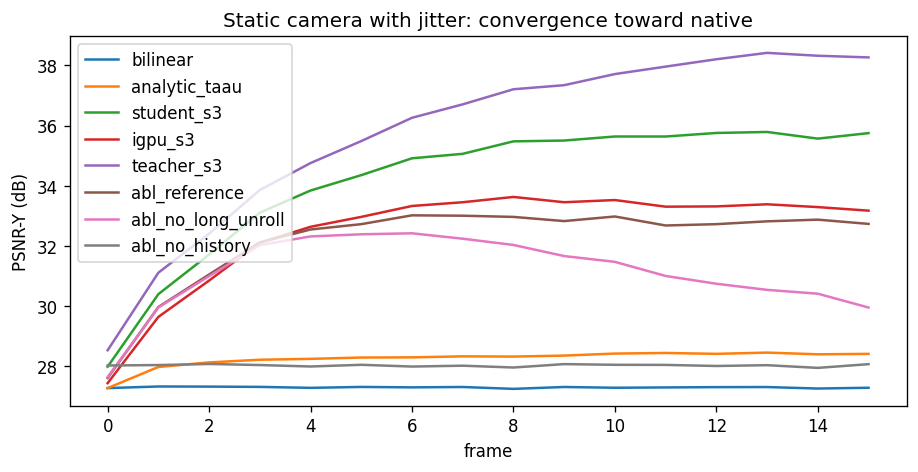
\includegraphics[width=\columnwidth]{fig-tsr-static.png}
\caption{Static camera with sub-pixel jitter on the synthetic suite: PSNR-Y against frame index for the baselines, the trained tiers and three ablations }\label{fig:static}
\end{figure}

\emph{Ablations.} \Cref{tab:tsr-abl} isolates the components with ablation runs of the \tier{low} recipe. History and G-buffers are the largest engine-mode effects (\ResAbsDiff{tsr.ablations.tartanair.engine.abl_no_history.psnr_y}{tsr.ablations.tartanair.engine.abl_reference.psnr_y} to \ResAbsDiff{tsr.ablations.vid4.engine.abl_no_history.psnr_y}{tsr.ablations.vid4.engine.abl_reference.psnr_y} dB). Plain-video training is worth \ResAbsDiff{tsr.ablations.tartanair.plain.abl_no_video_training.psnr_y}{tsr.ablations.tartanair.plain.abl_reference.psnr_y} to \ResAbsDiff{tsr.ablations.synthetic-game.plain.abl_no_video_training.psnr_y}{tsr.ablations.synthetic-game.plain.abl_reference.psnr_y} dB on plain video and costs nothing measurable on render input, where the model without it is \ResAbsDiff{tsr.ablations.tartanair.engine.abl_no_video_training.psnr_y}{tsr.ablations.tartanair.engine.abl_reference.psnr_y} to \ResAbsDiff{tsr.ablations.synthetic-game.engine.abl_no_video_training.psnr_y}{tsr.ablations.synthetic-game.engine.abl_reference.psnr_y} dB better. The motion estimator adds \ResAbsDiff{tsr.ablations.synthetic-game.plain.abl_no_motion_net.psnr_y}{tsr.ablations.synthetic-game.plain.abl_reference.psnr_y} to \ResAbsDiff{tsr.ablations.vid4.plain.abl_no_motion_net.psnr_y}{tsr.ablations.vid4.plain.abl_reference.psnr_y} dB on plain video. An earlier repeat with shorter budgets gave test means within a few tenths of a dB of these, so effects that size are noise. \Cref{fig:vid4} shows Vid4 in plain mode.

\begin{figure}[!t]
\centering
\setlength{\tabcolsep}{1pt}
\begin{tabular}{cc}
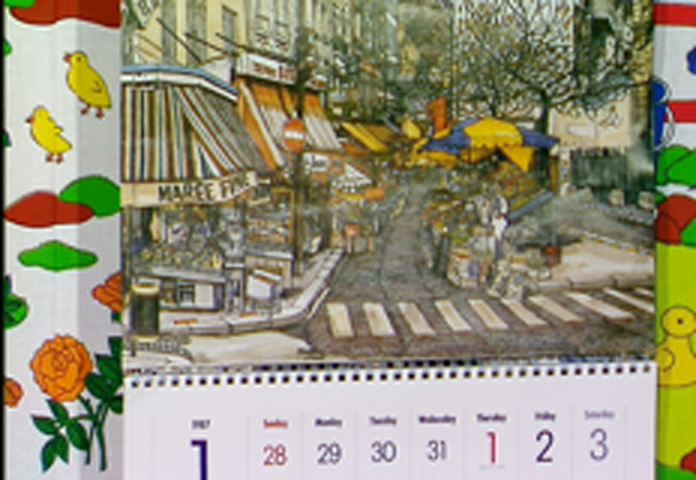
\includegraphics[width=0.48\columnwidth]{fig-tsr-vid4-bicubic.png} & 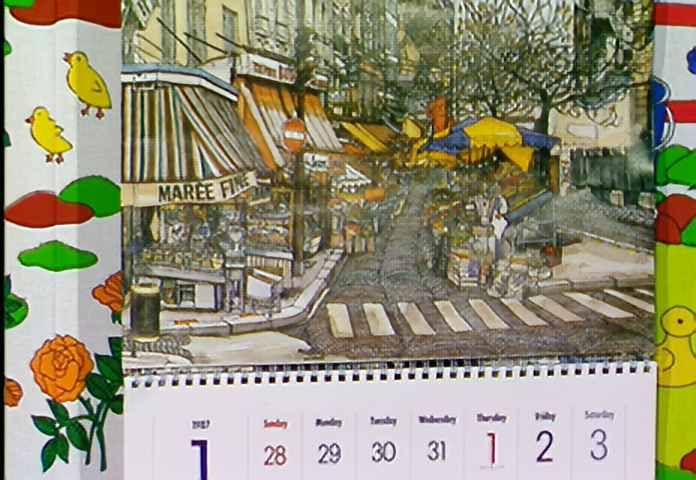
\includegraphics[width=0.48\columnwidth]{fig-tsr-vid4-student.png} \\
\footnotesize (a) Bicubic & \footnotesize (b) \tier{low} student \\
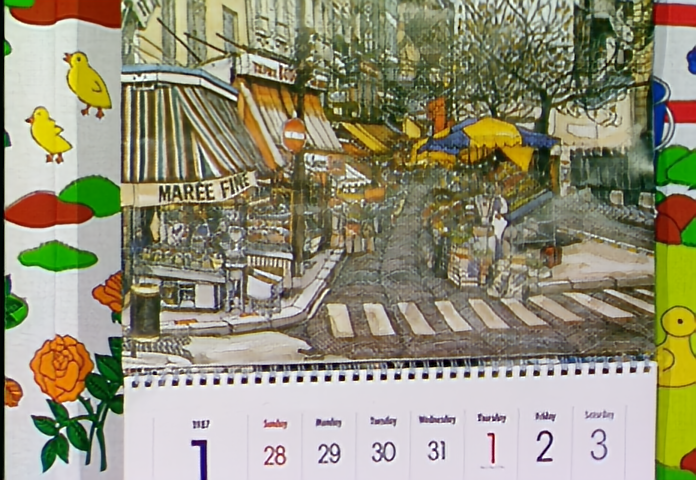
\includegraphics[width=0.48\columnwidth]{fig-tsr-vid4-teacher.png} & 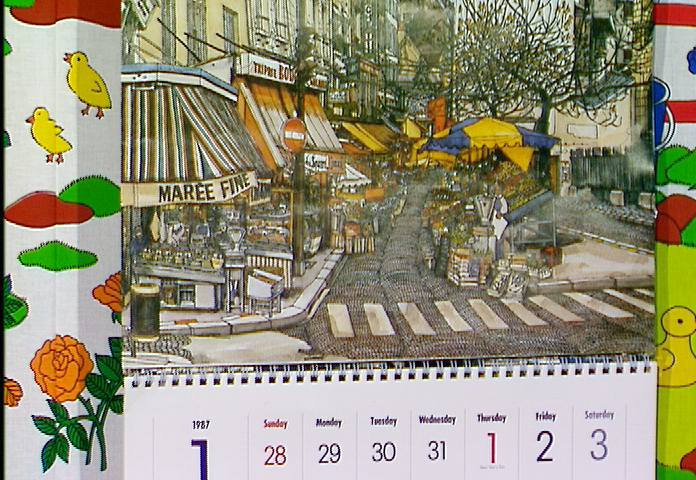
\includegraphics[width=0.48\columnwidth]{fig-tsr-vid4-ground-truth.png} \\
\footnotesize (c) Teacher & \footnotesize (d) Ground truth \\
\end{tabular}
\caption{Vid4 calendar at 3x in plain mode (bicubic downscale, no motion vectors). The student sharpens the sign lettering, awning stripes and calendar digits that bicubic upscaling blurs, but adds a fine grid texture on the cobblestones, and the teacher recovers more detail}\label{fig:vid4}
\end{figure}

\begin{figure*}[!t]
\centering
\setlength{\tabcolsep}{1pt}
\begin{tabular}{cccccc}
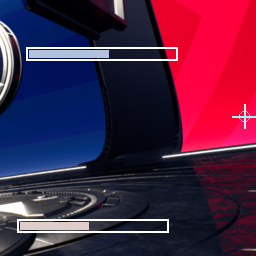
\includegraphics[width=0.16\textwidth]{fig-fg-ui-target.png} &
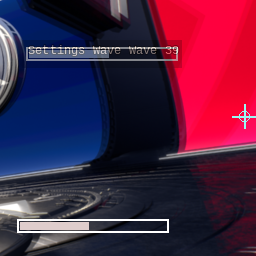
\includegraphics[width=0.16\textwidth]{fig-fg-ui-average.png} &
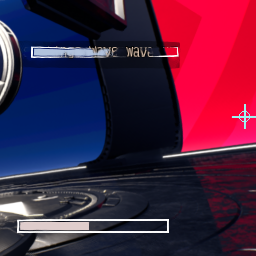
\includegraphics[width=0.16\textwidth]{fig-fg-ui-rife.png} &
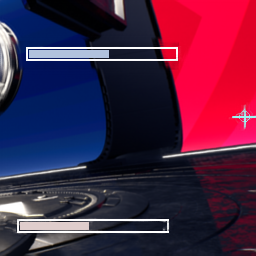
\includegraphics[width=0.16\textwidth]{fig-fg-ui-student.png} &
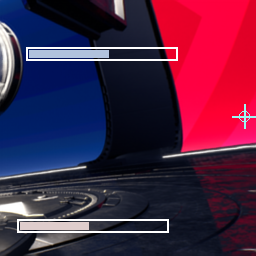
\includegraphics[width=0.16\textwidth]{fig-fg-ui-student-ui-layer.png} &
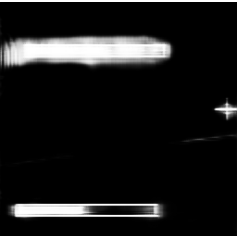
\includegraphics[width=0.16\textwidth]{fig-fg-ui-mask.png} \\
\footnotesize (a) Target & \footnotesize (b) Average & \footnotesize (c) RIFE 4.26 & \footnotesize (d) \tier{low} & \footnotesize (e) \tier{low} + UI layer & \footnotesize (f) Predicted UI mask \\
\end{tabular}
\caption{Interpolation of a synthetic scene with HUD bars, a crosshair and a changing subtitle. Averaging and RIFE blend the old and new subtitle text, the \tier{low} tier pulls the UI region towards the newest real frame using its predicted UI mask (f)}\label{fig:ui}
\end{figure*}

\subsection{Frame generation}\label{sec:res-fg}

\emph{Interpolation.} \Cref{tab:fg-interp} compares the tiers with RIFE 4.26 on plain video (Online Resource 1, \cref{S-sec:fgr-interp-plain,S-sec:fgr-mb}). The fine-tuned \tier{high} tier beats RIFE on Middlebury (\ResDiff{mb.middlebury_psnr.mean.high.psnr}{mb.middlebury_psnr.mean.rife_4_26.psnr} dB) and on four of the six video suites, by \ResAbsDiff{fg.test_per_sample.vimeo1080p.interp.plain.high.psnr}{fg.test_per_sample.vimeo1080p.interp.plain.rife_4_26.psnr} to \ResAbsDiff{fg.test_per_sample.vid4.interp.plain.high.psnr}{fg.test_per_sample.vid4.interp.plain.rife_4_26.psnr} dB. It ties on TartanAir (\ResDiff{fg.test_per_sample.tartanair.interp.plain.high.psnr}{fg.test_per_sample.tartanair.interp.plain.rife_4_26.psnr} dB) and loses \ResAbsDiff{fg.test_per_sample.sintel.interp.plain.high.psnr}{fg.test_per_sample.sintel.interp.plain.rife_4_26.psnr} dB on the \Res{fg.test_per_sample.sintel.interp.plain.kept} Sintel samples. The \tier{mid} tier (\Res{fg.model_tiers.mid.gmac_per_1080p_frame} GMAC) is within 0.5 dB of RIFE on every suite except TartanAir and Sintel. The \tier{low} tier beats frame averaging everywhere but trails RIFE by \ResAbsDiff{fg.test_per_sample.vid4.interp.plain.student.psnr}{fg.test_per_sample.vid4.interp.plain.rife_4_26.psnr} to \ResAbsDiff{fg.test_per_sample.tartanair.interp.plain.student.psnr}{fg.test_per_sample.tartanair.interp.plain.rife_4_26.psnr} dB. Engine hints change the interpolation PSNR of \tier{high} by \ResDiff{fg.test_results.sintel.interp.engine.high.psnr}{fg.test_results.sintel.interp.plain.high.psnr} dB on Sintel and \ResDiff{fg.test_results.tartanair.interp.engine.high.psnr}{fg.test_results.tartanair.interp.plain.high.psnr} dB on TartanAir (exact motion). Against RIFE 4.26 without hints, the hinted \tier{high} ranges from \ResDiff{fg.test_results.sintel.interp.engine.high.psnr}{fg.test_results.sintel.interp.plain.rife_4_26.psnr} dB on Sintel to \ResDiff{fg.test_results.tartanair.interp.engine.high.psnr}{fg.test_results.tartanair.interp.plain.rife_4_26.psnr} dB on TartanAir. In 3x multi-frame generation \tier{high} matches or beats RIFE on most suites, including Vimeo-1080p (\Res{fg.test_results.vimeo1080p.mfg3x.plain.high.psnr} against \Res{fg.test_results.vimeo1080p.mfg3x.plain.rife_4_26.psnr} dB) and native 1080p (\Res{fg.test_results.vimeo1080p_native.mfg3x.plain.high.psnr} against \Res{fg.test_results.vimeo1080p_native.mfg3x.plain.rife_4_26.psnr} dB).

\begin{table*}[!t]
\caption{FG interpolation on plain video (no engine hints), PSNR (dB). Video suites use samples the cut gate left alone (count in brackets). Middlebury was measured after the run on CPU with the downloaded weights. Bold marks the best method per row}\label{tab:fg-interp}
\begin{tabular*}{\textwidth}{@{\extracolsep\fill}lrrrrrr}
\toprule
Suite & Average & RIFE 4.26 & \tier{igpu} & \tier{low} & \tier{mid} & \tier{high} \\
\midrule
Middlebury (\Res{mb.middlebury_psnr.sequences}) & \Res{mb.middlebury_psnr.mean.average.psnr} & \Res{mb.middlebury_psnr.mean.rife_4_26.psnr} & \Res{mb.middlebury_psnr.mean.igpu.psnr} & \Res{mb.middlebury_psnr.mean.low.psnr} & \Res{mb.middlebury_psnr.mean.mid.psnr} & \textbf{\Res{mb.middlebury_psnr.mean.high.psnr}} \\
Vimeo-90K triplet (\Res{fg.test_per_sample.vimeo_triplet.interp.plain.kept}) & \Res{fg.test_per_sample.vimeo_triplet.interp.plain.average.psnr} & \Res{fg.test_per_sample.vimeo_triplet.interp.plain.rife_4_26.psnr} & \Res{fg.test_per_sample.vimeo_triplet.interp.plain.igpu.psnr} & \Res{fg.test_per_sample.vimeo_triplet.interp.plain.student.psnr} & \Res{fg.test_per_sample.vimeo_triplet.interp.plain.mid.psnr} & \textbf{\Res{fg.test_per_sample.vimeo_triplet.interp.plain.high.psnr}} \\
Vimeo-1080p, 544 lines (\Res{fg.test_per_sample.vimeo1080p.interp.plain.kept}) & \Res{fg.test_per_sample.vimeo1080p.interp.plain.average.psnr} & \Res{fg.test_per_sample.vimeo1080p.interp.plain.rife_4_26.psnr} & \Res{fg.test_per_sample.vimeo1080p.interp.plain.igpu.psnr} & \Res{fg.test_per_sample.vimeo1080p.interp.plain.student.psnr} & \Res{fg.test_per_sample.vimeo1080p.interp.plain.mid.psnr} & \textbf{\Res{fg.test_per_sample.vimeo1080p.interp.plain.high.psnr}} \\
Vimeo-1080p, native 1072 lines (\Res{fg.test_per_sample.vimeo1080p_native.interp.plain.kept}) & \Res{fg.test_per_sample.vimeo1080p_native.interp.plain.average.psnr} & \Res{fg.test_per_sample.vimeo1080p_native.interp.plain.rife_4_26.psnr} & \Res{fg.test_per_sample.vimeo1080p_native.interp.plain.igpu.psnr} & \Res{fg.test_per_sample.vimeo1080p_native.interp.plain.student.psnr} & \Res{fg.test_per_sample.vimeo1080p_native.interp.plain.mid.psnr} & \textbf{\Res{fg.test_per_sample.vimeo1080p_native.interp.plain.high.psnr}} \\
Vid4 (\Res{fg.test_per_sample.vid4.interp.plain.kept}) & \Res{fg.test_per_sample.vid4.interp.plain.average.psnr} & \Res{fg.test_per_sample.vid4.interp.plain.rife_4_26.psnr} & \Res{fg.test_per_sample.vid4.interp.plain.igpu.psnr} & \Res{fg.test_per_sample.vid4.interp.plain.student.psnr} & \Res{fg.test_per_sample.vid4.interp.plain.mid.psnr} & \textbf{\Res{fg.test_per_sample.vid4.interp.plain.high.psnr}} \\
TartanAir (\Res{fg.test_per_sample.tartanair.interp.plain.kept}) & \Res{fg.test_per_sample.tartanair.interp.plain.average.psnr} & \textbf{\Res{fg.test_per_sample.tartanair.interp.plain.rife_4_26.psnr}} & \Res{fg.test_per_sample.tartanair.interp.plain.igpu.psnr} & \Res{fg.test_per_sample.tartanair.interp.plain.student.psnr} & \Res{fg.test_per_sample.tartanair.interp.plain.mid.psnr} & \Res{fg.test_per_sample.tartanair.interp.plain.high.psnr} \\
Sintel (\Res{fg.test_per_sample.sintel.interp.plain.kept}) & \Res{fg.test_per_sample.sintel.interp.plain.average.psnr} & \textbf{\Res{fg.test_per_sample.sintel.interp.plain.rife_4_26.psnr}} & \Res{fg.test_per_sample.sintel.interp.plain.igpu.psnr} & \Res{fg.test_per_sample.sintel.interp.plain.student.psnr} & \Res{fg.test_per_sample.sintel.interp.plain.mid.psnr} & \Res{fg.test_per_sample.sintel.interp.plain.high.psnr} \\
\botrule
\end{tabular*}
\end{table*}

\emph{Extrapolation.} \Cref{tab:fg-extrap} shows the mode that adds no held frame (Online Resource 1, \cref{S-sec:fgr-extrap}). RIFE is not built for $\tau>1$: it is below frame repetition on Vimeo-1080p and native 1080p, and at most \ResAbsDiff{fg.test_per_sample.vid4.extrap.plain.rife_4_26.psnr}{fg.test_per_sample.vid4.extrap.plain.repeat.psnr} dB above it on the others. On plain video \tier{high} beats repetition by \ResAbsDiff{fg.test_per_sample.vimeo1080p_native.extrap.plain.high.psnr}{fg.test_per_sample.vimeo1080p_native.extrap.plain.repeat.psnr} to \ResAbsDiff{fg.test_per_sample.tartanair.extrap.plain.high.psnr}{fg.test_per_sample.tartanair.extrap.plain.repeat.psnr} dB, and \tier{low} by \ResAbsDiff{fg.test_per_sample.vimeo1080p_native.extrap.plain.student.psnr}{fg.test_per_sample.vimeo1080p_native.extrap.plain.repeat.psnr} to \ResAbsDiff{fg.test_per_sample.tartanair.extrap.plain.student.psnr}{fg.test_per_sample.tartanair.extrap.plain.repeat.psnr} dB. With engine motion vectors, motion-vector reprojection remains better on TartanAir (\ResAbsDiff{fg.test_per_sample.tartanair.extrap.engine.high.psnr}{fg.test_per_sample.tartanair.extrap.engine.mv_reprojection.psnr} dB, exact motion).

\begin{table}[!t]
\caption{FG extrapolation ($\tau=1.5$), PSNR (dB), samples the cut gate left alone. Plain: no engine hints. Engine: with motion vectors, depth and camera prior, against motion-vector reprojection (MV)}\label{tab:fg-extrap}
\begin{tabular*}{\columnwidth}{@{\extracolsep\fill}lrrrr}
\toprule
Plain & Repeat & RIFE & \tier{low} & \tier{high} \\
\midrule
Vimeo-1080p & \Res{fg.test_per_sample.vimeo1080p.extrap.plain.repeat.psnr} & \Res{fg.test_per_sample.vimeo1080p.extrap.plain.rife_4_26.psnr} & \Res{fg.test_per_sample.vimeo1080p.extrap.plain.student.psnr} & \textbf{\Res{fg.test_per_sample.vimeo1080p.extrap.plain.high.psnr}} \\
Native 1080p & \Res{fg.test_per_sample.vimeo1080p_native.extrap.plain.repeat.psnr} & \Res{fg.test_per_sample.vimeo1080p_native.extrap.plain.rife_4_26.psnr} & \Res{fg.test_per_sample.vimeo1080p_native.extrap.plain.student.psnr} & \textbf{\Res{fg.test_per_sample.vimeo1080p_native.extrap.plain.high.psnr}} \\
Vid4 & \Res{fg.test_per_sample.vid4.extrap.plain.repeat.psnr} & \Res{fg.test_per_sample.vid4.extrap.plain.rife_4_26.psnr} & \Res{fg.test_per_sample.vid4.extrap.plain.student.psnr} & \textbf{\Res{fg.test_per_sample.vid4.extrap.plain.high.psnr}} \\
TartanAir & \Res{fg.test_per_sample.tartanair.extrap.plain.repeat.psnr} & \Res{fg.test_per_sample.tartanair.extrap.plain.rife_4_26.psnr} & \Res{fg.test_per_sample.tartanair.extrap.plain.student.psnr} & \textbf{\Res{fg.test_per_sample.tartanair.extrap.plain.high.psnr}} \\
Sintel & \Res{fg.test_per_sample.sintel.extrap.plain.repeat.psnr} & \Res{fg.test_per_sample.sintel.extrap.plain.rife_4_26.psnr} & \Res{fg.test_per_sample.sintel.extrap.plain.student.psnr} & \textbf{\Res{fg.test_per_sample.sintel.extrap.plain.high.psnr}} \\
\midrule
Engine & MV & & \tier{low} & \tier{high} \\
\midrule
Vimeo-1080p & \Res{fg.test_per_sample.vimeo1080p.extrap.engine.mv_reprojection.psnr} & & \Res{fg.test_per_sample.vimeo1080p.extrap.engine.student.psnr} & \textbf{\Res{fg.test_per_sample.vimeo1080p.extrap.engine.high.psnr}} \\
Native 1080p & \Res{fg.test_per_sample.vimeo1080p_native.extrap.engine.mv_reprojection.psnr} & & \Res{fg.test_per_sample.vimeo1080p_native.extrap.engine.student.psnr} & \textbf{\Res{fg.test_per_sample.vimeo1080p_native.extrap.engine.high.psnr}} \\
Vid4 & \Res{fg.test_per_sample.vid4.extrap.engine.mv_reprojection.psnr} & & \Res{fg.test_per_sample.vid4.extrap.engine.student.psnr} & \textbf{\Res{fg.test_per_sample.vid4.extrap.engine.high.psnr}} \\
TartanAir & \textbf{\Res{fg.test_per_sample.tartanair.extrap.engine.mv_reprojection.psnr}} & & \Res{fg.test_per_sample.tartanair.extrap.engine.student.psnr} & \Res{fg.test_per_sample.tartanair.extrap.engine.high.psnr} \\
Sintel & \textbf{\Res{fg.test_per_sample.sintel.extrap.engine.mv_reprojection.psnr}} & & \Res{fg.test_per_sample.sintel.extrap.engine.student.psnr} & \Res{fg.test_per_sample.sintel.extrap.engine.high.psnr} \\
Synthetic & \Res{fg.test_per_sample.synthetic.extrap.engine.mv_reprojection.psnr} & & \Res{fg.test_per_sample.synthetic.extrap.engine.student.psnr} & \textbf{\Res{fg.test_per_sample.synthetic.extrap.engine.high.psnr}} \\
\botrule
\end{tabular*}
\end{table}

\emph{UI, camera reversal and cuts.} On synthetic HUD and subtitle scenes (interpolation with engine hints) the UI ghosting rate is \Res{fg.ui_results.interp.engine.student.ui_ghost_rate} for \tier{low} and \Res{fg.ui_results.interp.engine.high.ui_ghost_rate} for \tier{high}, against \Res{fg.ui_results.interp.engine.rife_4_26.ui_ghost_rate} for RIFE and \Res{fg.ui_results.interp.engine.mv_reprojection.ui_ghost_rate} for reprojection, and \Res{fg.ui_results.interp.engine.student_ui_layer.ui_ghost_rate} when the engine supplies a UI layer (\cref{fig:ui}). Removing UI training raises it to \Res{fg.ui_results.interp.engine.abl_no_ui_training.ui_ghost_rate}. On rapid camera reversals in extrapolation the late-latched camera prior raises \tier{low} from \Res{fg.camera_prior.synthetic-reversal.extrap.engine.prior_off.student.psnr.mean} to \Res{fg.camera_prior.synthetic-reversal.extrap.engine.prior_on.student.psnr.mean} dB and \tier{high} from \Res{fg.camera_prior.synthetic-reversal.extrap.engine.prior_off.high.psnr.mean} to \Res{fg.camera_prior.synthetic-reversal.extrap.engine.prior_on.high.psnr.mean} dB, while repetition scores \Res{fg.camera_prior.synthetic-reversal.extrap.engine.prior_on.repeat.psnr.mean} dB (Online Resource 1, \cref{S-sec:fgr-reversal}). The gate detected all \Res{fg.cut_gate_rates.synthetic-cut.interp.engine.samples} synthetic cuts in both input modes. With motion vectors it false-alarmed on \ResRatio{fg.cut_gate_rates.vimeo1080p.interp.engine.gated}{fg.cut_gate_rates.vimeo1080p.interp.engine.samples} of the Vimeo-1080p samples and \ResRatio{fg.cut_gate_rates.sintel.interp.engine.gated}{fg.cut_gate_rates.sintel.interp.engine.samples} of the Sintel samples, and on none of the TartanAir, Vid4 and native 1080p samples. Without them it false-alarmed on \ResRatio{fg.cut_gate_rates.vid4.interp.plain.gated}{fg.cut_gate_rates.vid4.interp.plain.samples} to \ResRatio{fg.cut_gate_rates.vimeo1080p.interp.plain.gated}{fg.cut_gate_rates.vimeo1080p.interp.plain.samples} of two-frame real samples, on \ResRatio{fg.cut_gate_rates.tartanair.mfg3x.plain.gated}{fg.cut_gate_rates.tartanair.mfg3x.plain.samples} to \ResRatio{fg.cut_gate_rates.sintel.mfg3x.plain.gated}{fg.cut_gate_rates.sintel.mfg3x.plain.samples} of the 3x multi-frame samples in four suites (none on Vid4), whose real frames are three apart, and on \ResRatio{fg.cut_gate_rates.synthetic.interp.plain.gated}{fg.cut_gate_rates.synthetic.interp.plain.samples} of continuous synthetic pairs, against a calibration target of 0.01.
\emph{Ablations.} Ablation runs of the \tier{low} recipe show that the RIFE weights matter most on plain video: without inheritance Vimeo-90K interpolation drops from \Res{fg.ablations.vimeo_triplet.interp.plain.abl_reference.psnr} to \Res{fg.ablations.vimeo_triplet.interp.plain.abl_no_inheritance.psnr} dB (Online Resource 1, \cref{S-sec:fgr-abl}). Without engine hints in training, extrapolation with exact motion on TartanAir falls from \Res{fg.ablations.tartanair.extrap.engine.abl_reference.psnr} to \Res{fg.ablations.tartanair.extrap.engine.abl_no_motion_prior.psnr} dB, but plain-video interpolation rises from \Res{fg.ablations.vimeo_triplet.interp.plain.abl_reference.psnr} to \Res{fg.ablations.vimeo_triplet.interp.plain.abl_no_motion_prior.psnr} dB. A model trained only for extrapolation fails at interpolation (\Res{fg.ablations.vimeo_triplet.interp.engine.abl_extrap_only.psnr} against \Res{fg.ablations.vimeo_triplet.interp.engine.abl_reference.psnr} dB with engine hints).

\subsection{Real-time cost}\label{sec:res-time}

\Cref{tab:tiers} gives the measured T4 times (Online Resource 1, \cref{S-sec:fgr-latency}). They are far above the arithmetic cost: the \Res{fg.model_tiers.low.gmac_per_1080p_frame}-GMAC FG \tier{low} tier takes \Res{fg.latency.student.1920x1080.t4_mean_ms} ms and the \Res{tsr.model_tiers.igpu.3.gmac_per_frame_1080p}-GMAC TSR \tier{igpu} tier \Res{tsr.latency.igpu_s3.3.1920x1080.t4_mean_ms} ms. The \tier{mid} and \tier{high} FG tiers are faster at 1440p (\Res{fg.latency.mid.2560x1440.t4_mean_ms} and \Res{fg.latency.high.2560x1440.t4_mean_ms} ms) than at 1080p (\Res{fg.latency.mid.1920x1080.t4_mean_ms} and \Res{fg.latency.high.1920x1080.t4_mean_ms} ms) because their flow is halved above 1152 lines. With \Res{fg.latency.student.1920x1080.t4_mean_ms} ms per generated frame, the pacing model at a 30 fps render rate drops the displayed rate to \Res{fg.pacing_model.interp.33_3.displayed_fps} fps in every FG mode. Interpolation raises game latency from \Res{fg.pacing_model.native.33_3.game_latency_ms} to \Res{fg.pacing_model.interp.33_3.game_latency_ms} ms, while extrapolation keeps it at \Res{fg.pacing_model.extrap.33_3.game_latency_ms} ms and late latching brings camera latency to \Res{fg.pacing_model.extrap_late.33_3.camera_latency_ms} ms. The fused networks export to ONNX with a maximum ONNX Runtime difference of \Res{tsr.onnx_export.0.ort_max_abs} (TSR) and \Res{fg.onnx_export.0.ort_max_abs} (FG). The graphs are static: the FG graph for a $128\times128$ input and the TSR graph for a $36\times64$ render, so another size needs a new export.

\section{Discussion}\label{sec:discussion}

\emph{What one model per task achieves.} A single TSR network handles jittered renders with engine data and plain video without it. Training on both degradations is what makes plain video work, and it costs the render path nothing measurable (\cref{tab:tsr-abl}). Longer budgets did not help in the earlier repeat, so the next TSR gains need more exact-motion data rather than more time. For FG, fine-tuning RIFE 4.26 with zero-initialised hints keeps its quality and adds extrapolation, UI handling and a camera prior.

\emph{Where it falls short.} The tiers that fit integrated and entry GPUs do not reach RIFE 4.26's quality in FG. The \tier{low} tier stays \ResAbsDiff{mb.middlebury_psnr.mean.low.psnr}{mb.middlebury_psnr.mean.rife_4_26.psnr} dB below RIFE on Middlebury, with half of RIFE's channel widths and \ResRatio{fg.model_tiers.low.gmac_per_1080p_frame}{fg.model_tiers.high.gmac_per_1080p_frame} of its cost, so capacity now limits it. Extrapolation with exact motion vectors does not beat plain reprojection on TartanAir. The histogram cut gate is not deployable. Most importantly for real-time use, every measured tier exceeds a 16.7 ms frame budget in eager PyTorch on a T4 except the TSR \tier{igpu} tier, which takes \Res{tsr.latency.igpu_s3.3.1920x1080.t4_mean_ms} ms (\Res{tsr.latency.igpu_s3.3.1920x1080.t4_mean_ms_engine_mv} ms with engine motion vectors), nearly the whole budget. The TSR \tier{low} tier's \Res{tsr.latency.student_s3.3.1920x1080.t4_mean_ms} ms is \ResRatio{tsr.latency.student_s3.3.1920x1080.t4_mean_ms}{tsr.latency.student_s3.3.1920x1080.est_ms_assumed_igpu_4_tflops_fp16_sustained} times its arithmetic estimate for a 4-TFLOPS integrated GPU, which points to per-kernel overhead and memory traffic. We infer this from the timings and have not profiled it.

\emph{Threats to validity.} Each configuration ran once, and only the TSR configuration was repeated with other budgets (Online Resource 1, \cref{S-sec:status-limits}). Several ungated FG means rest on few samples (\Res{fg.test_per_sample.vid4.interp.plain.kept} Vid4 and \Res{fg.test_per_sample.vimeo1080p_native.interp.plain.kept} native 1080p samples). Vimeo-90K makes up \ResRatio{tsr.caches.window_sources.train.vimeo_septuplet}{tsr.caches.caches.seq_train.count} of the real TSR training windows, and only the Sintel and TartanAir windows have exact motion. Low-resolution inputs are simulated from finished frames, so level-of-detail, shading-rate and lighting effects of real renderers are missing. The plain-video protocol uses clean bicubic downscaling, while real video adds codec artefacts. We did not compare with commercial upscalers or frame generators, which needs engine captures, and latency was measured on a data-centre GPU, not on target hardware.

\section{Conclusion}\label{sec:conclusion}

\Sys{} shows that one compact recurrent network can upscale both engine renders and plain video, beating bicubic and analytic TAA upscaling on five suites, and that fine-tuning RIFE 4.26 with zero-initialised engine hints yields a frame generator that beats RIFE at its own width while adding extrapolation, UI handling and a camera prior. The results also mark what remains: the \tier{low} and \tier{igpu} frame-generation tiers are \ResAbsDiff{fg.test_per_sample.vid4.interp.plain.student.psnr}{fg.test_per_sample.vid4.interp.plain.rife_4_26.psnr} to \ResAbsDiff{fg.test_per_sample.tartanair.interp.plain.student.psnr}{fg.test_per_sample.tartanair.interp.plain.rife_4_26.psnr} and \ResAbsDiff{fg.test_per_sample.vid4.interp.plain.igpu.psnr}{fg.test_per_sample.vid4.interp.plain.rife_4_26.psnr} to \ResAbsDiff{fg.test_per_sample.tartanair.interp.plain.igpu.psnr}{fg.test_per_sample.tartanair.interp.plain.rife_4_26.psnr} dB below RIFE in plain interpolation, cut detection without motion vectors false-alarms, and in eager execution only the smallest super-resolution tier fits a 60 fps frame budget, with almost no margin. Next steps are wider half-resolution-flow FG tiers, cut thresholds calibrated on real clips per frame gap, deployment runtimes timed on integrated GPUs, repeated seeds, and engine captures for a comparison with commercial systems.

\backmatter

\section*{Statements and Declarations}\label{sec:declarations}
\pdfbookmark[1]{Statements and Declarations}{declarations}

\bmhead{Supplementary information} Online Resource 1 (supplementary material) explains every component, equation, training objective and evaluation protocol from first principles and presents every table, plot and prediction of the three notebooks with its interpretation. Its references carry the prefix S.

\bmhead{Funding} No funding was received for this work.

\bmhead{Competing interests} The author has no competing interests to declare.

\bmhead{Data availability} All datasets are public: DIV2K, Flickr2K, REDS, Vimeo-90K, Vid4 and MPI Sintel on Kaggle, and TartanAir, the CARLA-based GameIR renders, 1080p game frames and Vimeo-1080p on Hugging Face. The dataset identifiers, the split manifest, every metric file, plot and log of the runs reported here\ifdefined\Anonymised{} are available from the corresponding author and will be released with the code on acceptance.\else{} are in the project repository, \RepoURL.\fi

\bmhead{Code availability} \ifdefined\Anonymised The code, notebooks and trained weights will be released on acceptance.\else The code, the three Kaggle notebooks with their executed outputs and the trained weights are in the same repository.\fi

\bmhead{Ethics approval and consent} Not applicable.

\bmhead{Author contributions} \ifdefined\Anonymised Withheld for review.\else Parth Mital designed the system, ran the experiments, analysed the results and wrote the manuscript.\fi

\ifdefined\NoReferences\else
\pdfbookmark[1]{References}{references}
\fi
\bibliography{references}

\end{document}
